
\chapter{Introduction} \label{Intro}

pySixDesk is a novel platform for managing massive simulations using sixtrack  which is a single particle tracking code widely used at CERN. It allows to set up and manage job submission, gather results and analyse them. pySixDesk comes as a python library, hence, it can be imported into a python terminal or into custom-made python scripts.

The pySixDesk package could be obtained from github repository:

\url{https://github.com/SixTrack/pysixdesk}


\paragraph{The requirements:}~

The native environment of pySixDesk is CERN's lxplus login service;The guidelines in the following will assume that this is the case.
\begin{enumerate}
    \item AFS and openAFS for disk storage;
    \item kerberos for login and user identification;
    \item htcondor, as batch service native at CERN;
    \item BOINC, as additional batch service for long-term, large simulation campaigns;
    \item sqlite, for the database monitoring the progress of jobs and storing data;
    \item mysql, the central database service used to store data;
    \item python3, as main language.
\end{enumerate}

% ================================================================================================================================ %

\paragraph{Shell set-up}~

It is recommended to use pySixDesk from the python shell. Please remember to use python3. On lxplus, python3 is available as python3 command, since the default python command uses version 2.7.5.

In order to use the library, it is essential to declare in your live python environment the path where the pysixdesk package can be found. This can be accomplished adding the path to the pysixdesk package to the PYTHONPATH environment variable (in the following, \$pysixdesk\_path is the full path to pysixdesk),eg:

\begin{lstlisting}
export PYTHON=$PYTHONPATH:$pysixdesk_path/
\end{lstlisting}

or to add it to the sys.path list, e.g:

\begin{lstlisting}[language=Python]
import sys
sys.path.append(<path_to_pysixdesk>/)
\end{lstlisting}

\section{Workflow of a study}

In pysixdesk, the program will start from a configuration file named 'config.py'. It contains all the necessary parameters needed by the jobs, such as database type, name of template file, pathes of madx and sixtrack executable, boinc spool directory, scan parameters for sixtrack and so on.

Due to the input files of an acutal sixtrack job are generated by madx, so the progress is divided into two parts. The first part is called preprocess job which will execute madx to generate input files for sixtrack, and other steps such as one-turn job for DA study, merge aperture node into fort.2 for collimation study. The second part is the sixtrack job which will execute the actual sixtrack job. 
\paragraph{preprocess jobs}~

All the studies will start from a single *.mask file. The mask file has some placeholders to generate the actual madx input files by replacing the placeholders with the given values.
\begin{lstlisting}
.....
! A Laundau octupole current 20A inj, -570A col
I_MO=%OCT;

!General switch to select collision (0/1)
ON_COLLISION:=0;
!General switch to install bb lens (0/1)
ON_BB_SWITCH:=0;
......
\end{lstlisting}

For the upper example, the user should set 'self.madx\_params['OCT'] = 0' in the config file to generate an acutal madx input file.

The program will create the actual madx input file and execute madx to generate files for sixtrack jobs. In general, they will be 'fc.2', 'fc.3', 'fc.8', 'fc.16'. If the user is working on dynamic aperture (DA) study, the one-turn sixtrack job is needed to get the twiss-parameters, 
\begin{figure}[h]
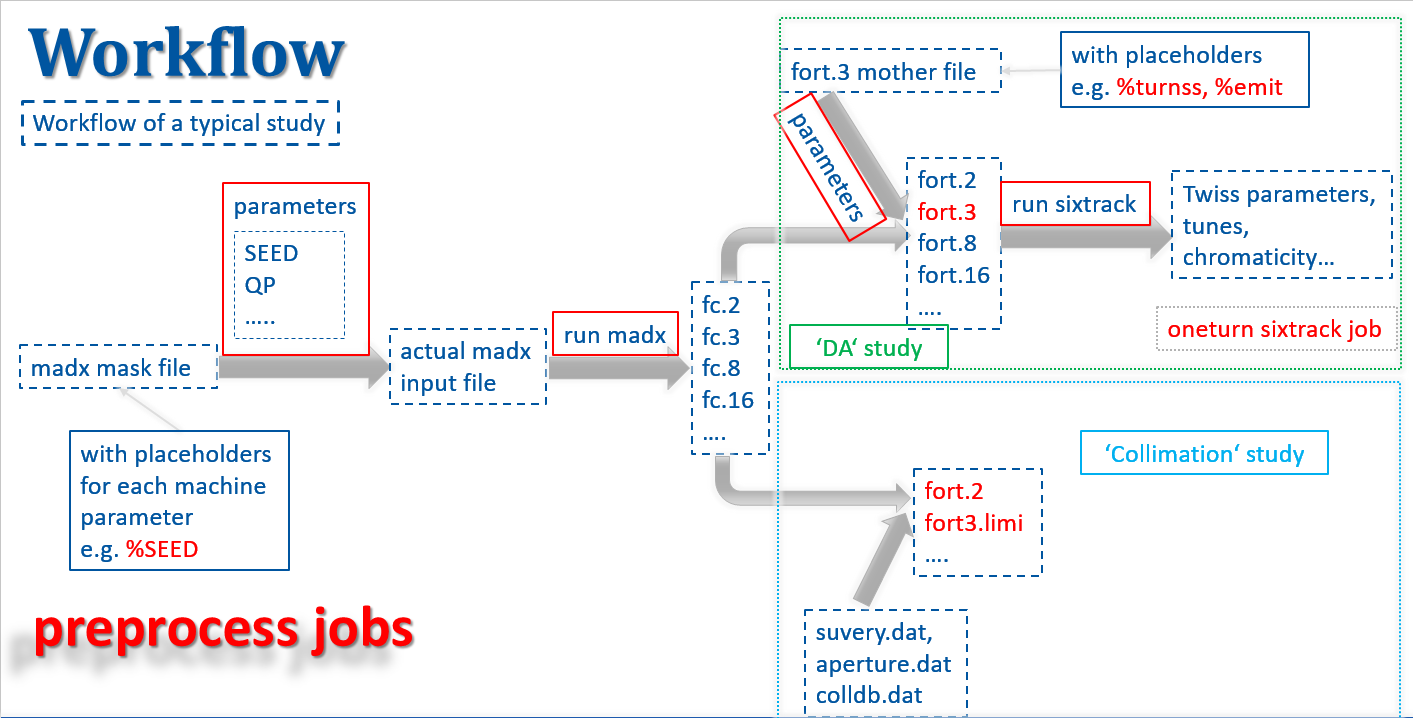
\includegraphics[width=17cm]{preprocess.png}
\caption{The workflow of preprocess job}
\label{fig1}
\centering
\end{figure}

\paragraph{sixtrack job}~

\begin{figure}[h]
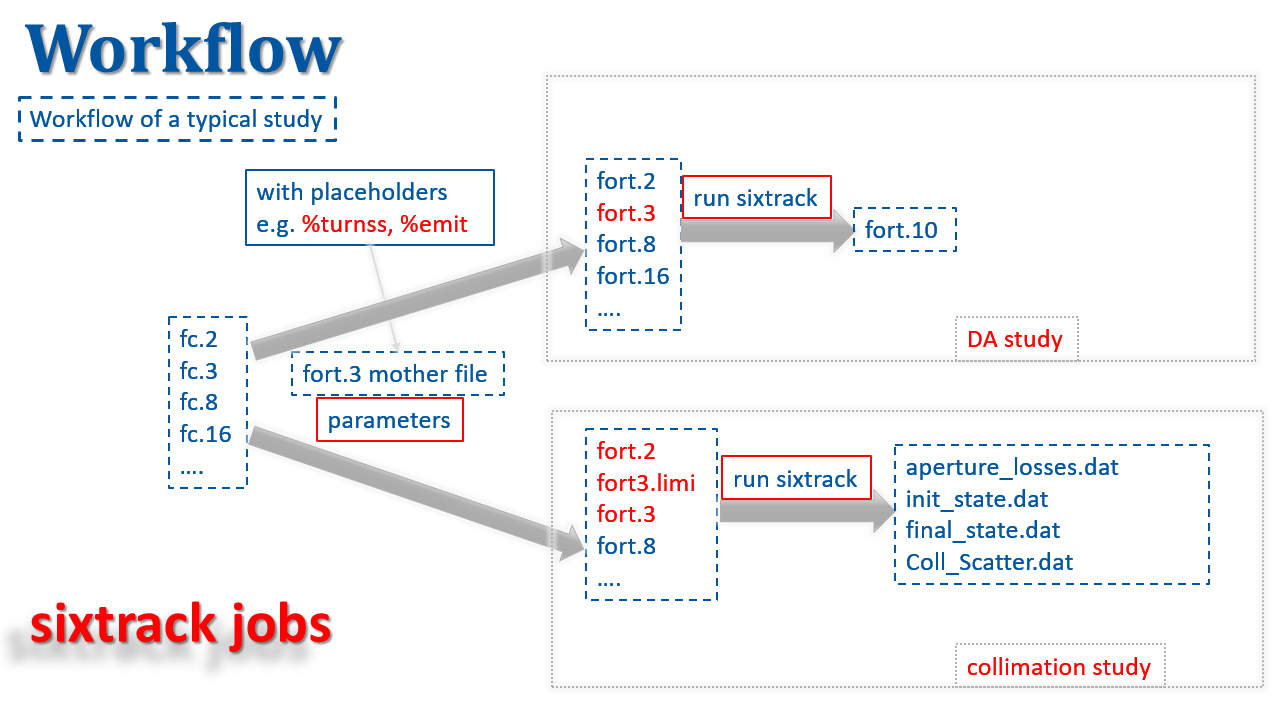
\includegraphics[width=17cm]{sixtrack.png}
\caption{The workflow of sixtrack job}
\label{fig2}
\centering
\end{figure}

\section{Database}

In pySixDesk, sqlite3 and mysql are employed as the main databases to store the data. sqlite3 is the local file-based db, and mysql is the server-based db. For sqlite3 database, it will sit in your study path with an unified name \textbf{data.db}, and for mysql database, we use the DB-On-Demand server which is managed by CERN IT.
  To connect to mysql, the username, password, host, port are needed at least. For security reason, the \textbf{config.py} doesn't hold these information, the user should prepare a config file \textbf{.my.cnf} under the home directory \textbf{(\$HOME)} which contains the information, it looks like:
\begin{lstlisting}
[client]
user = test1
password = test
host = 127.0.0.1
port = 3306
\end{lstlisting}

Below is a scalability test result for different databases. The test condition: 300 preprocess jobs, 30000 sixtrackjobs. All operations were done on CERN lxplus and all jobs were submitted to HTCondor.
\begin{table}[h]
    \caption{Scalability tests for these two databases.}
    \label{T-ExtRou}
    \centering
    \renewcommand{\arraystretch}{1.5}
    \begin{tabular}{|l|l|l|}
        \hline
        \rowcolor{blue!30}
        \textbf{Action/DB} & \textbf{Sqlite3} & \textbf{Mysql} \\
        \hline
        \texttt{setup DB}  & 5s & 11s \\
        \hline
        \texttt{prepare preprocess}  & 1s & 1s \\
        \hline
        \texttt{submit}   & 6s    & 27s \\
        \hline
        \texttt{collection}   & 120s   & - \\
        \hline
        \texttt{prepare sixtrack}  & 240s & 128s \\
        \hline
        \texttt{submit}   & 435s    & 294s \\
        \hline
        \texttt{collection}   & ~3h   & - \\
        \hline
    \end{tabular}
\end{table}

Where '-' represent no need.
Note that if the user select mysql and submit jobs to BOINC, the collection process is still needed. For the moment, the volunteer computers can't access to the mysql server directly.

%\subsection{Command Line Arguments} \label{sec:cmdarg}
%
%SixTrack does not require any command line arguments, but can optionally take the file name for the main input file as well as the geometry file as the first and second argument, respectively.
%See also Sections~\ref{InFiles} and~\ref{ProVer}.
%
%\bigskip
%\noindent In addition, SixTrack can echo the version number and exit with the following flags:
%\begin{itemize}
%    \item[\texttt{-v}] Echo program name and version as a single line, and exit.
%    \item[\texttt{-V}] Echo program name, version, release date, and git hash on four lines, and exit.
%    \item[\texttt{-nv}] Echo the numerical version as an integer, and exit,
%\end{itemize}
